\documentclass[12pt, letterpaper]{article}
\usepackage[utf8]{inputenc}
\usepackage[english]{babel}
\usepackage{fancyhdr}
\usepackage{geometry}
\usepackage{natbib}
\bibliographystyle{besjournals}
%\addbibresource{references.bib}
\newcommand{\pkg}[1]{{\fontseries{b}\selectfont #1}}
\usepackage{booktabs, tabularx, longtable}
\usepackage{array}
\usepackage{colortbl}
\usepackage{graphicx}
\graphicspath{ {./figures/} }
\usepackage[section]{placeins}
\usepackage{amsmath}
\usepackage[leftcaption]{sidecap}

%try to deal with issue of figures going to the end of the document
\makeatletter
\AtBeginDocument{%
  \expandafter\renewcommand\expandafter\subsection\expandafter{%
    \expandafter\@fb@secFB\subsection
  }
}
\makeatother

\geometry{margin = 1in}
\pagestyle{fancy}
\fancyhf{}
%set the header
\rhead{\thepage}
\lhead{A.Stears}
%set the line spacing
\renewcommand{\baselinestretch}{1.5}
%add line numbers
\usepackage{lineno}
\linenumbers

% Add additional packages here if required
\usepackage{siunitx}
\usepackage{authblk}

\title{Functional traits %be specific about which functional traits
mediate the effect of climate variation on plant demographic rates in shortgrass steppe ecosystems}
\author[1]{Alice Stears}
\author[2]{Peter Adler}
\author[3]{Dana Blumenthal} %ask Dana if there are any additional authors we should include-- i.e. Kevin Mueller?
\author[3]{Julie Kray}
\author[4]{Troy Ocheltree}
\author[5]{Kevin Wilcox}
\author[1]{Daniel C. Laughlin}

% Include full affiliation details for all authors
\affil[1]{Botany Department and Program in Ecology, University of Wyoming, Laramie, WY}
\affil[2]{Department of Wildland Resources and the Ecology Center, Utah State University, Logan, UT}
\affil[3]{USDA-ARS Rangeland Resources Research Unit, Fort Collins, CO}
\affil[5]{Department of Ecosystem Science and Management, University of Wyoming, Laramie, WY}
\affil[4]{Warner College of Natural Resources, Colorado State University, Fort Collins, CO}

\begin{document}

\begin{flushleft}
\Large{\textbf{Functional traits mediate the effect of climate variation on plant demographic rates in a shortgrass steppe ecosystem}}

\normalsize{Alice E. Stears$^{1*}$, Peter B. Adler$^2$, Dana M. Blumenthal$^3$, Julie A. Kray$^4$, Troy W. Ocheltree$^5$, Kevin R. Wilcox$^5$, Daniel C. Laughlin$^1$}

\small{$^1$Botany Department and Program in Ecology, University of Wyoming, Laramie, WY; $^2$Department of Wildland Resources and the Ecology Center, Utah State University, Logan, UT; $^3$USDA-ARS Rangeland Resources Research Unit, Fort Collins, CO, $^4$Warner College of Natural Resources, Colorado State University, Fort Collins, CO, $^5$Department of Ecosystem Science and Management, University of Wyoming, Laramie, WY}

\small{$^*$Corresponding Author, astears@uwyo.edu}
\end{flushleft}


\begin{abstract}
\begin{enumerate}
\item Global climate change increases the likelihood of extreme weather events and exacerbates variability in inter-annual climate.  This heightened variation in weather will affect biodiversity and ecosystem function. Previous work has characterized broad relationships between plant traits and regional climate, but this work has largely ignored the population underlying community structure. 
\item We determine how the impact of plant functional traits on growth and survival depends on inter-annual drought variation. We synthesized 15 years of demographic data, species-level morphological and physiological functional trait measurements, and records of annual climate variability in a short-grass steppe ecosystem in northern Colorado (COSGS).  We also calculated the Standardized Precipitation Evapotranspiration Index (SPEI) for each growing season as a measure of drought intensity. We fit Generalized Linear Mixed Effect Models that account for the effect of plant size and local neighborhood competition to determine whether traits interact with growing-season water availability to impact growth and survival.
\item We predict that turgor loss point (TLP), a trait directly related to water use, will best predict changes in plant growth and survival in response to drought. Low TLP species will have a higher probability of growth and survival in dry years than high TLP species. Leaf dry matter content (LDMC) will also predict demographic responses to drought, since plants with higher rates of carbon allocation to leaf structure (higher LDMC) will be more resistant to wilting. 
\item  The impact of trait on survival varies significantly across a gradient of SPEI for TLP (P = 0.018), LDMC (P $<$ 0.05), and root dry matter content (RDMC) (P $<$ 0.05). Individuals with more negative TLP and higher LDMC and RDMC had higher survival rates in drier years, while the inverse is true in wet years. LDMC and RDMC, morphological traits, have a stronger interactive effective effect with SPEI on survival than TLP, a physiological trait. This contradicts our predictions, and might indicate that leaf and root structural integrity, measured by LDMC and RDMC,  is more important than osmotic maintenance (measured by TLP) for maintaining turgid leaves under water stress.  We identified neither a direct nor an interactive effect of any functional trait on growth, which suggests that drought is a strong filter in this system, and plants that survive drought have mechanisms to avoid or withstand the negative effect of water stress on growth.   
\item \textit{Synthesis} These results emphasize the importance of considering environmental variation when evaluating the impact of traits on demographic rates. This work also suggests that morphological traits such as LDMC and RDMC are better than physiological traits at predicting drought tolerance in this system, which indicates further study of drought tolerance mechanisms employed by species in shortgrass steppe. Finally, this more nuanced understanding of the relationship between traits, water availability, and survival provides a tool for refining predictions of how shortgrass steppe will respond to more intense and frequent drought in the future.  
\end{enumerate}
\end{abstract}

\section{Introduction}

Intro Draft Outline using CARS model
-
As the frequency and severity of extreme climate events increases with climate change, it becomes increasingly important to understand how plant populations and communities will respond. While the impacts of global change may be most clearly expressed at the population and community levels, these changes are largely driven by the effects of environmental variation on individual-level processes such as growth and survival. It is critical, then, to understand how extreme climate variation impacts these vital rate processes. Individual characteristics such as plant size and age, as well as biotic effects such as competition, have a known impact on the way demographic rates respond to abiotic variation \citep{Adler2012, Tredennick2018}. We also know that demographic rates differ in their impact on population dynamics for different broad plant categories. For example,  survival is more important for long-lived species, while growth and reproduction are more important for short-lived species \citep{Adler2014}. However, we lack a generalizable understanding of which traits interact with the environment to alter plant demographic rates, and thus fitness \citep{Laughlin2018}(Fig. \ref{fig:ConceptFig}) Here, we identify how plant functional traits related to water use impact species growth and survival across a temporal gradient of water availability in a Colorado shortgrass steppe ecosystem. 

Physiological measurements that are good predictors of drought tolerance such as leaf hydraulic conductance or leaf turgor loss point (TLP), are labor intensive and impractical to assess across many individuals or species. However, recent methodological advances have made some physiological traits such as TLP easier to measure. Osmometer-based estimates of leaf osmotic potential at full turgor have been shown to be tightly correlated with leaf TLP, and this trait is suggested to be a good predictor of drought tolerance in woody species \citep{Bartlett2012}. Subsequent work has shown that leaf osmotic potential is also tightly linked with leaf TLP in herbaceous species in western North American grasslands, and is correlated with traits with established links to drought tolerance \citep{Griffin-Nolan2019}. Previous work has linked leaf TLP to leaf-level drought tolerance, as well as drought tolerance measured via species occurrence across gradients of water availability \citep{Bartlett2012a,Blumenthal2020,Wilcox2020PlantPrairie}.
However the extent to which TLP variation mediates the effect of drought on plant demographic rates is not known. Despite advances in method, traits such as leaf dry matter content (LDMC) and root dry matter content (RDMC) are still easier to measure, and may be as good as physiological measurements at predicting drought tolerance across a gradient of water availability\citep{Bartlett2012,Griffin-Nolan2019,Blumenthal2020}.

We determine if species-level functional trait measurements can improve our predictions of plant survival probability and growth across a gradient of drought severity. To accomplish this goal, we integrate long-term demographic data from chart-quadrats, climate records, and species-level trait measurements to develop statistical models that quantify how traits predict survival and growth, and how the nature of that relationship changes according to inter-annual drought severity. 
%explain hypotheses for individual traits/why they are included in this study
Species that we expect to be drought tolerant (high LDMC, low TLP) should have higher survival probability in dry years than species with low LDMC and high TLP (Fig. \ref{fig:PredsObs}) Additionally, we predict that physiological traits related to water use (TLP) and morphological functional traits that are related to water content and growth rate (LDMC) will be better predictors of survival in response to drought in comparison to other traits such as SLA that are correlated with leaf economic strategy \citep{Wright2004, Reich2014}. Like SLA, LDMC is correlated with plant relative growth rate and resource-acquisition strategy \citep{Weiher1999ChallengingEcology}, but is a more direct measurement of leaf structure and allocation of carbon to leaf tissue than SLA \citep{Niinemets1999ComponentsPlants,Hodgson2011}. Species with higher LDMC have higher allocation to cell wall structure and more densely-packed leaf cells, and thus are more likely to maintain cell turgor under water stress \citep{Niinemets2001Global-scaleShrubs,Poorter2009CausesMeta-analysis,Wilcox2020PlantPrairie}.%having a hard time finding literature to support a hypothesis about RDMC... am I using a search term that is incorrect? (i.e. should I be searching on something different from "root dry matter content?" 
We also expect that physiological traits will be stronger predictors of survival than easy-to-measure functional traits, since they are more direct measurements of physiological processes that impact growth and survival. 
\begin{figure}
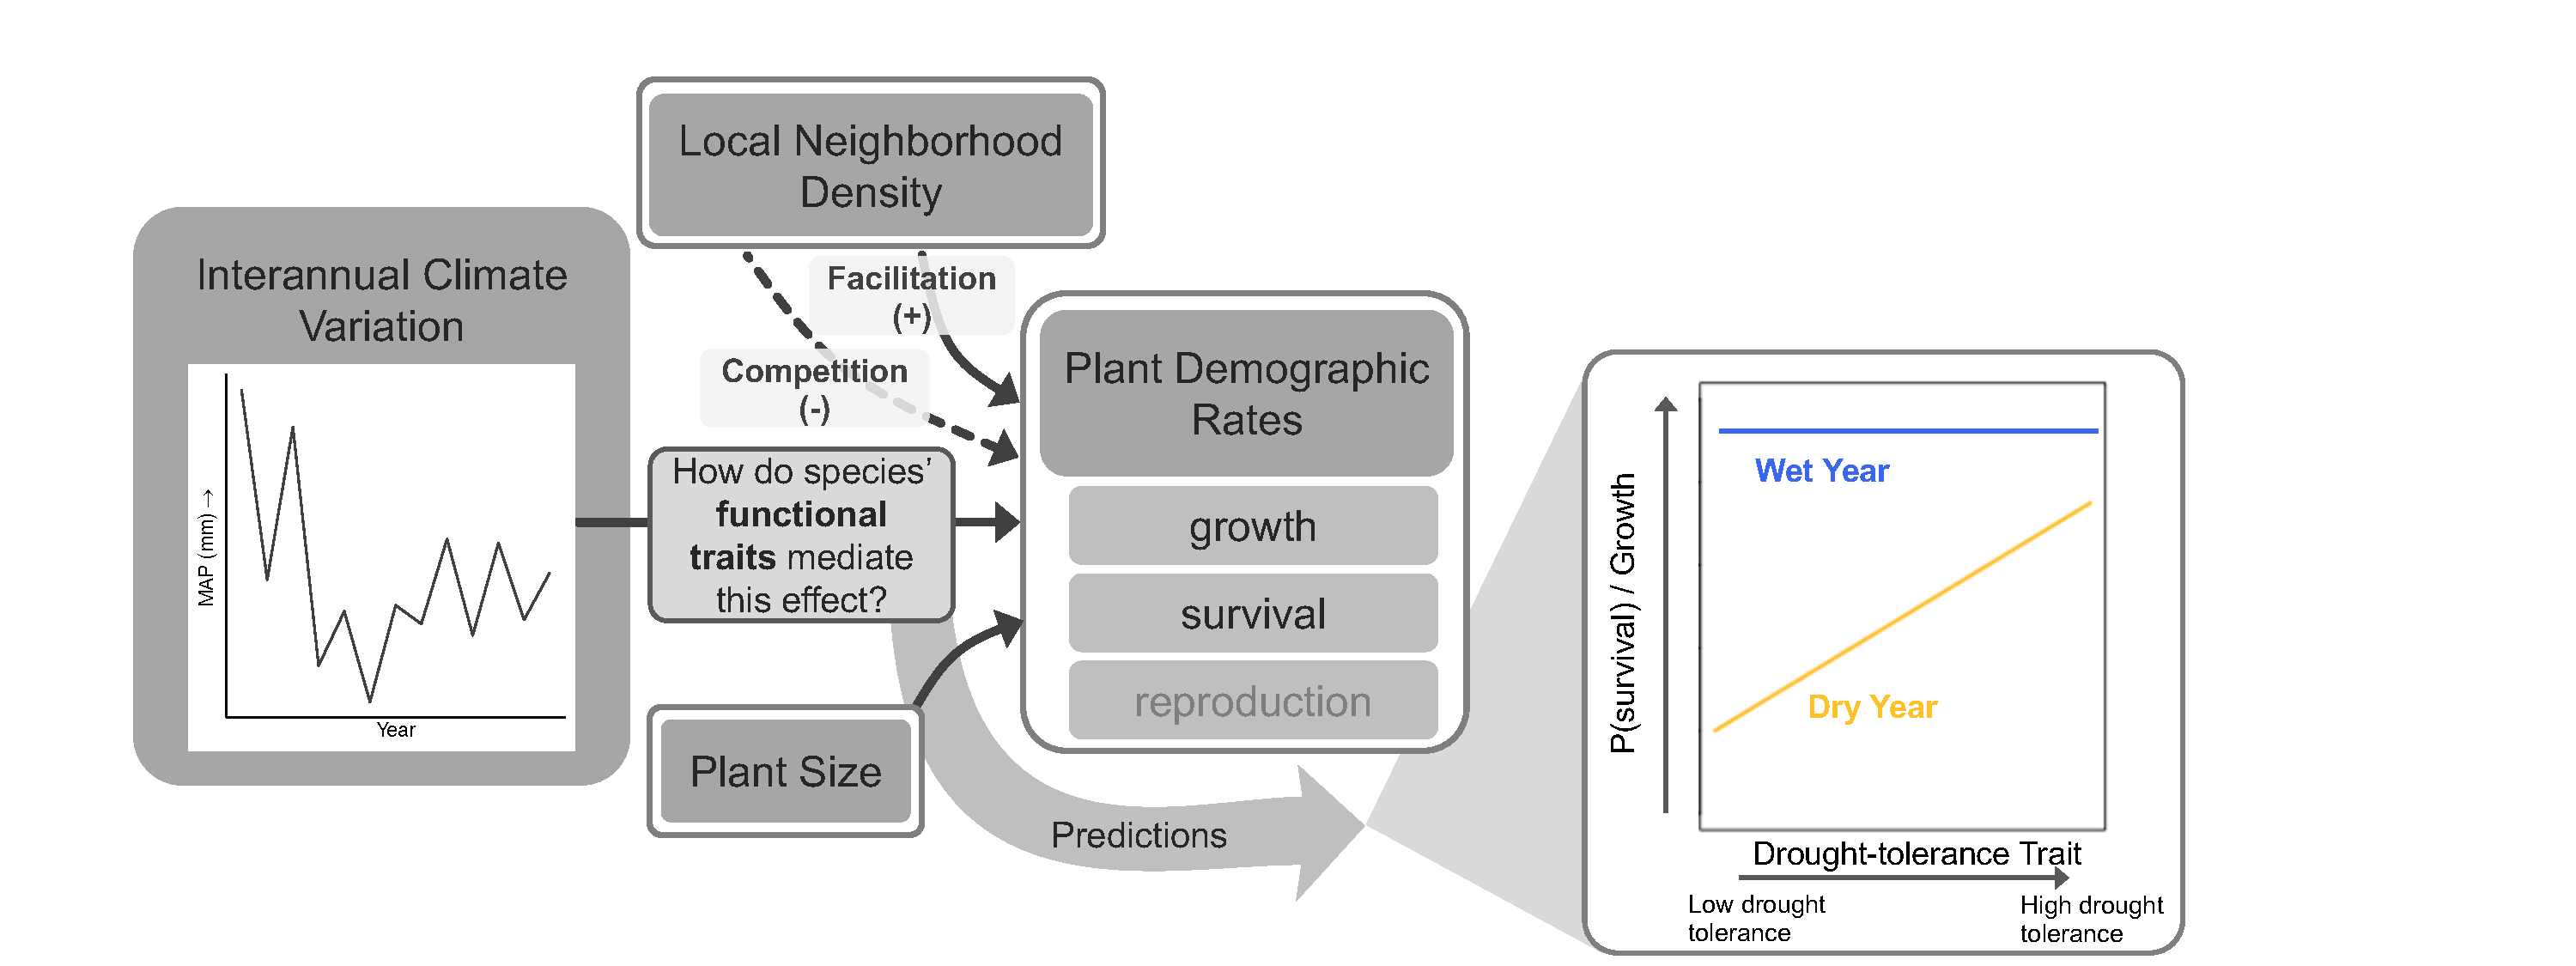
\includegraphics[width=1\textwidth]{figures/CO_sgs_ConceptualFigure.pdf}
\caption{\small{
The demographic processes of growth, survival, and reproduction, which can also be referred to as 'demographic rates', are impacted by environmental variation, interactions with neighboring organisms, and plant size. Due to limitations of our dataset, we focus here on growth and survival and do not investigate reproduction. The impact of environmental variation on an organism's demographic rates is likely mediated by the functional traits of that organism. This is especially likely for traits that are related to environmental covariates that are most limiting or stress-inducing in a given habitat. For example, traits related to water use might be more important for plant growth and survival in very dry years, and relatively less important in years with high water availability. The 'Predictions' panel shows how a drought-tolerance related functional trait might mediate the effect of climate on growth and survival. A species' trait value is important for determining survival or growth probability in dry years, but is not important in wet years when a plant is not experiencing severe water stress. 
}}
\label{fig:ConceptFig}
\end{figure}

\section{Methods}
\subsection{Demographic Data} 
We monitored growth and survival for eight graminoid and eight forb species for 13 continuous annual transitions over 24, 1-m$^2$ chart-quadrats at the Central Plains Experimental Research Location (CPER) in Nunn, Colorado, USA (40.8$^o$N/110.8$^o$W). These quadrats were established as part of the Shortgrass Steppe Long Term Ecological Research project \citep{Chu2013}. This site is located at 1650 m elevation in the North American shortgrass steppe, which is dominated by \textit{Bouteloua gracilis} and \textit{Bouteloua dactyloides}. It receives an average of 340 mm of precipitation annually, and has a mean annual temperature of 8 $^o$C \citep{Chu2014}. Soils at the CPER are primarily Mollisols and Aridisols.

The chart-quadrat method used does not assign each individual a unique identifying number or tag, but does map each individual plant in a spatially explicit manner each year. Bunchgrasses, shrubs, and other plants with a sizeable basal area were mapped as polygons, while grasses and forbs with a small number of stems were mapped as points. Of the species included in this analysis, graminoids are all measured as polygons, and forbs are all measured as points, so each data type will be referenced as either 'graminoids' or 'forbs.' Growth can only be extracted from this dataset for individuals measured as polygons, because size is not measured for points. We calculated growth as the difference between log(size$_{t+1}$) and log(size$_t$) for each individual.  

We extracted growth and survival data from a digitized version of this map dataset using "tracking algorithms" in R \citep{Lauenroth2008, RCoreTeam2019}. These algorithms loop through the annual maps for a given quadrat, and assume that individuals of the same species growing in the same location in consecutive years are the same individual. In this way, the algorithms generate records of survival for all species, and records of growth or shrinkage for species measured as polygons. These tracking algorithms allow a plant to go dormant for one year. This means that if an individual is present in year 1, absent from the maps in year 2, but present in year 3 at the same coordinates as year 1, this plant is considered to be the same individual. We also allow a 'buffer' of 5 cm in observations of the same individual from year to year, which accounts for measurement error as well as true variation in re-sprouting location across years. 
\subsection{Climate Data} The standardized precipitation-evapotranspiration index (SPEI) is a drought metric that uses temperature and precipitation data to estimate evapotranspiration and soil moisture \citep{Vicente-Serrano2010}.  To calculate SPEI for this analysis we used climate data from the Global SPEI database, which calculates SPEI at a 55 $km^2$ resolution \citep{Vicente-Serrano2010}. SPEI can be calculated over an interval as short as one month, or as long as 48 months. In this study, each species has a unique phenology and potentially reacts to timing of drought differently. Therefore, we calculated SPEI for each species using an SPEI interval that matches their growth interval. For example, for a species that grows and flowers from May through August, SPEI is calculated each year with a four month interval that ends in August. The beginning of the growth interval was assumed to be one month before the start of flowering. Flowering data was collected from a Colorado flora \citep{Ackerfield2015}.  
\subsection{Trait Data} We measured leaf and root functional traits for the graminoid, shrub, and forb species that comprise most of the diversity in the demographic dataset. Five to ten mature and healthy individuals of each target species were collected for each target species. A majority of the trait values used in this analysis come from samples collected at the demographic data collection site, the USDA-ARS CPER. Several other species were measured at USDA-ARS High Plains Grasslands Research Station (HPGRS) near Cheyenne, WY, a northern mixed-grass habitat. Samples for trait measurement were collected at CPER and HPGRS between 2014 and 2018 \citep{Blumenthal2020}. We supplemented this dataset with leaf and root trait data measured from samples collected at the University Pasture in Hays, KS (southern mixed-grass prairie), the USDA-ARS Ft. Keogh Livestock and Range Research Station in Miles City, MT (northern mixed-grass prairie), and the USDA-ARS US Sheep Experiment Station near Dubois, ID (sagebrush steppe). See (Table \ref{TraitMeasurements}) for a list of sampling locations for each species included in this analysis. 

We measured species-level average trait values for seven traits: specific leaf area (SLA; cm$^2$/g), leaf dry matter content (LDMC; g/g), turgor loss point (TLP; MPa), specific root length (SRL; g/m), average root diameter (RDiam; mm), root dry matter content (RDMC; g/g), and root tissue density (RTD; g/cm$^3$). SLA and LDMC were measured using standard methods \citep{Perez-Harguindeguy2013}. TLP was calculated from measurements of leaf osmotic potential made using a Vapro 5600 osmometer \citep{Bartlett2012, Griffin-Nolan2019}. TLP was derived from osmotic potential using the following equation: leaf turgor loss point $= 0.944($leaf osmotic potential$) - 0.611$. Below ground traits were measured for fine, absorptive root tissue (typically 1st-3rd order roots) \citep{McCormack2015}. Root length, average diameter, and root volume were measured using WinRhizo software.
\subsection{Statistical Analysis} 
We use a generalized linear mixed-effect (GLMM) model framework to identify how the effect of trait values on growth and survival varies across a spectrum of drought intensity. We also use this model framework to assess the relative ability of each trait to predict growth and survival. We used the \pkg{lme4} package in \textsf{R} to create GLMMs with a binomial error distribution and a logit link function, as well as random effects for species, quadrat, year, and plant size, to quantify the interactive effects of climate and trait values on \textbf{survival} \citep{RCoreTeam2019, Bates2015}. Individual size is an important covariate in these models, but is only available for graminoids because forbs were mapped as points in this dataset. Because of this, we modeled graminoid and forb survival separately, and forb models do not contain a size covariate or a random slope for size. We modeled the interactive effect of climate and traits on \textbf{growth} using a similar model framework to the one used for survival, but with a Gaussian error distribution. Growth models were only constructed for graminoids, since we do not have data showing growth for forbs because they were mapped as points. The global model structure for both growth and survival of graminoids and forbs followed this  general structure:

\begin{multline}
\label{surv_eq}
logit(survival)\;\mathbf{OR}\;size_{t+1}\sim \alpha + \gamma_{species}+ \delta_{quad} + \tau_{year} + size_t(\beta_{species}  + \beta_1) + trait\beta_2+ SPEI\beta_3\\ + nearEdge\beta_4  + neighborhoodDensity\beta_5 + trait\times SPEI\beta_6
\end{multline}
Survival models use a binary response variable indicating whether an individual survived (1) or died (0) in year t+1. Individual plant size in year t+1 is the response variable for growth models \citep{Dalgleish2011ClimatePlants, Dahlgren2009LinkingHerb}. In both model frameworks, the fixed effects of interest are SPEI, trait, and the SPEI-by-trait interaction. We created separate growth and survival models for each trait, since we are interested in the relative ability of each trait to predict drought tolerance along a gradient of SPEI. To account for the effects of individual plant size \citep{Tredennick2018} and competition on demographic rates (Fig.\ref{fig:ConceptFig}), we included individual plant basal area (when available) and conspecific local neighborhood density as fixed effect covariates in our models (Equation \ref{surv_eq}). Local neighborhood density, a metric that accounts for the effect of intra-specific competition or facilitation on demographic rates, is a value we calculated for each individual observation in the demographic data. For graminoids, the local neighborhood density is the total plant basal area within a 10 cm radius of the focal individual that is occupied by individuals of the same species (conspecifics). For forbs, this value is a sum of the total number of conspecific stems within a 10 cm local neighborhood radius of the focal individual. We tested different neighborhood radii (5, 10, 15, and 20 cm) to determine which radius is the most appropriate to use in this ecological context by fitting four generalized linear mixed-effect models for the effect of a trait-by-environment interaction on survival (following the framework of Equation \ref{surv_eq}) while including a competition metric using a different radius in each model. We compared the size of the coefficient for the fixed effect of competition in each model, and determined that the competition metric using a 10 cm radius was most appropriate because it was the largest. We chose to calculate only intra-specific competition estimates, since it has been shown that inter-specific competition is typically weak in dry grassland systems \citep{Adler2018}. We also included a fixed effect, "nearEdge," which is a binary variable indicating whether an individual was growing within 5 cm of the quadrat edge. This covariate accounts for the higher probability of 'missing' an edge individual during mapping, as well as potential under-estimation of local neighborhood density or individual size due to proximity to the quadrat edge. 

Growth and survival models for both graminoids and forbs included a random intercept for quadrat to account for spatial autocorrelation, and a random intercept for year to account for temporal autocorrelation. Because data on individual size was available for graminoids, we included a random slope for size associated with a random intercept for species, which accounts for the fact that larger individuals of a given species have a higher growth and survival probability than small individuals, but also allows for variation in maximum and minimum plant size for each species. We did not include a random slope for size according to species for RTD and SRL survival models and all growth models, since model fit was singular when this random slope was included \citep{Bates2015}. 
%how best to say this? 
Because individual size data is not available for forbs, we did not include a random slope for size in the forb survival models, but still included a random intercept for species to account for variation in trait-by-SPEI relationships across species.

We used AIC model selection to determine the best random effect structure for each model, and AIC model selection to determine the best fixed effect structure. To compare the extent to which including a trait increases the accuracy of a model that predicts survival probability, we compared the AIC of models that include a trait and trait-by-environment interaction to a model using the same data but without the trait and interaction term. The larger the decrease in AIC in the trait model relative to the no-trait model, the more support for the ability of that trait to predict survival or growth in response to drought.

\begin{figure}
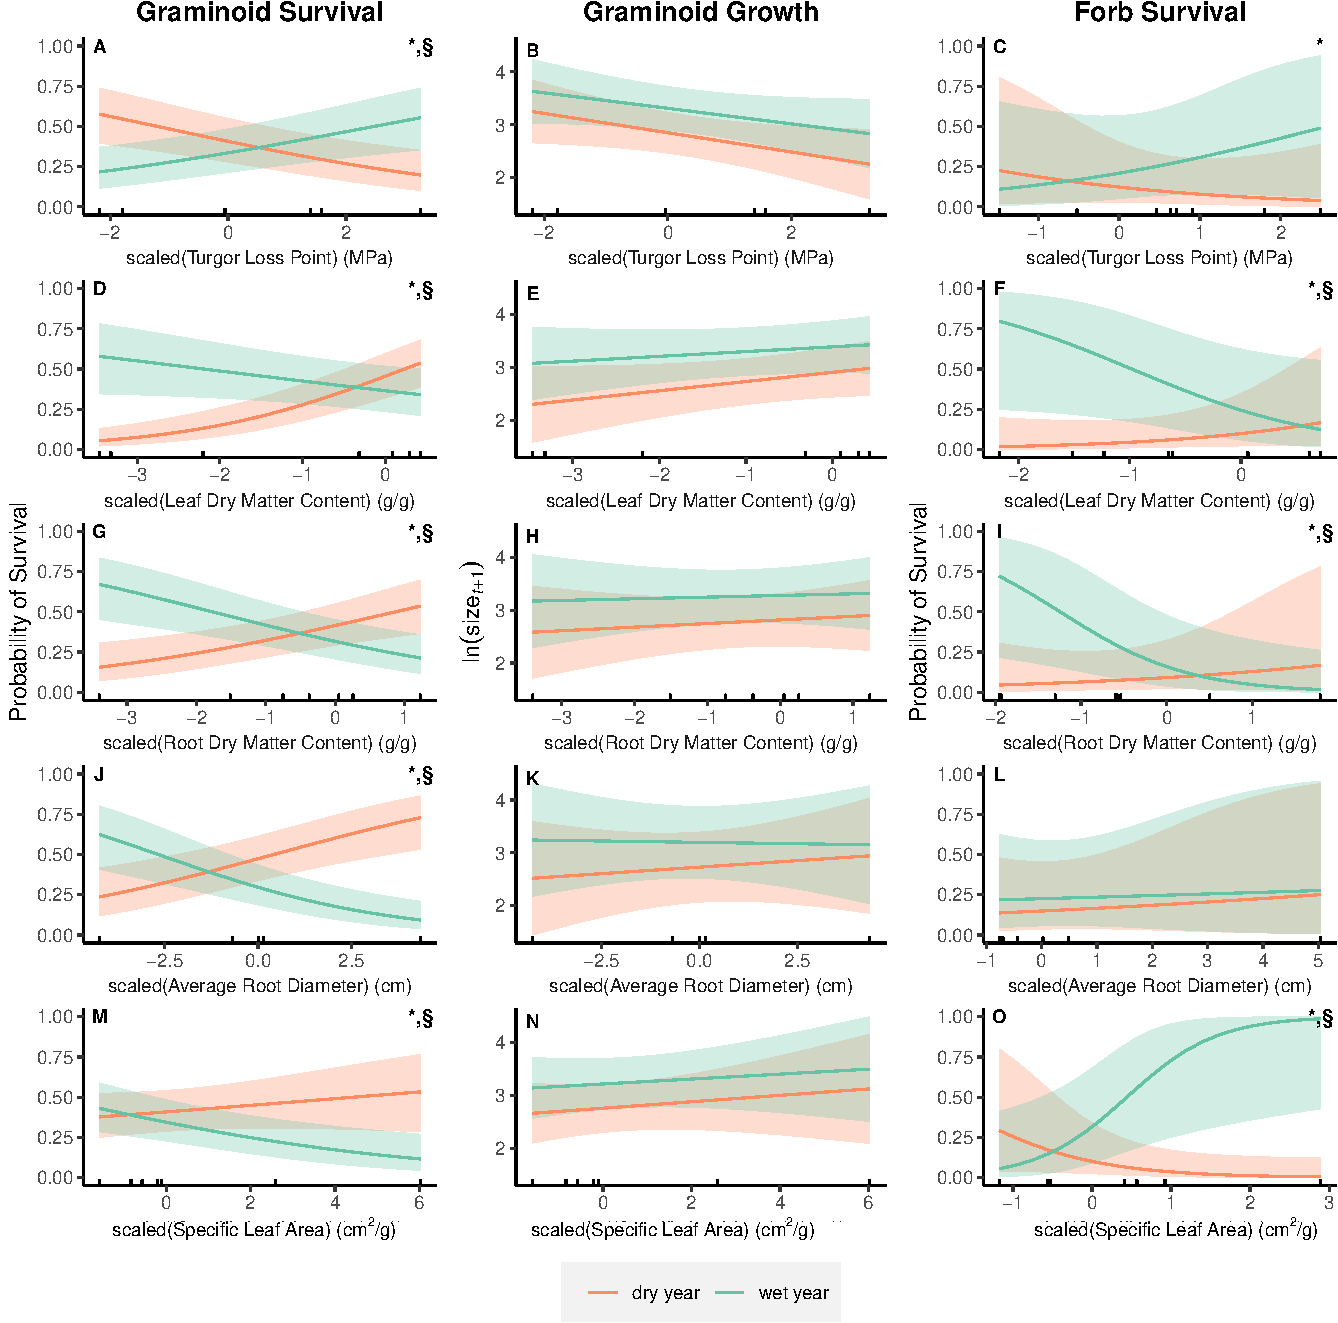
\includegraphics[width=.9\textwidth]{figures/mainObservationsFig-1.pdf}
\caption[width=0.35\textwidth]{\small{Predicted effect of Turgor Loss Point (\textbf{A}), Leaf Dry Matter Content (\textbf{B}), and Root Dry Matter Content (\textbf{C}) on the probability of survival in dry (yellow) and wet years (green). \textbf{D} Graminoid species are more likely to survive in dry years (low SPEI) if they have a low TLP than species with a high TLP, while species with a high TLP are slightly more likely to survive in wet years (high SPEI) (Marginal R$^2$ = 0.34, Conditional R$^2$ = 0.56; interaction term coefficient = 0.08, p $<$ 0.01). \textbf{E} A similar trend in graminoid survival probability is predicted by the model that includes LDMC (Marginal R$^2$ = 0.39, Conditional R$^2$ = 0.51; interaction term coefficient = -0.14, p $<$ 0.01). \textbf{F} A similar trend to LDMC exists for graminoid survival probability as predicted by the interaction between RDMC and SPEI (Marginal R$^2$ = 0.27, Conditional R$^2$ = 0.44; interaction term coefficient = -0.11, p $<$ 0.01)
\textbf{G}, \textbf{H}, and \textbf{I} show that similar trends were observed for forbs, although the model fit is weaker and the interaction between trait and environment is less significant for each trait (\textbf{G}: Marginal R$^2$ = 0.02, Conditional R$^2$ = 0.40; interaction term coefficient = 0.28, p = 0.02)(\textbf{H}: Marginal R$^2$ = 0.03, Conditional R$^2$ = 0.38; interaction term coefficient = -0.34, p = 0.01)(\textbf{I}: Marginal R$^2$ = 0.03, Conditional R$^2$ = 0.38; interaction term coefficient = -0.30, p = 0.02). Black vertical bars along the x-axis (rug plots) indicate the trait values of the species included in each analysis. Survival probability for 'wet years' and 'dry years' are calculated for the 97.5$^{th}$ and 2.5$^{th}$ quantiles of the distribution of SPEI values.
}}
\label{fig:PredsObs}
\end{figure}

\begin{table}[h] \centering 
  \caption{Trait Measurement Information} 
  \label{TraitMeasurements}
  \resizebox{\textwidth}{!}{%
\begin{tabular} {lccccccc|ccccc|cc} 
\\[-1.8ex]\hline 
\hline \\[-1.8ex] 
& \multicolumn{7}{c}{\textbf{Traits}} & \multicolumn{5}{c}{\textbf{Sampling Location}} & \multicolumn{2}{c}{\textbf{Func. Group}}\\
 & TLP & RootDiam & RTD & RDMC & SRL & LDMC & SLA & CPER & HPGRS & Sheep Station & Ft. Keogh  & Hays & Gram. & Forb\\ 
\hline \\[-1.8ex] 
\rowcolor[gray]{.95} \textit{Bouteloua gracilis} & $\times$ & $\times$ & $\times$ & $\times$ & $\times$ & $\times$ & $\times$ & $\times$ &&&&&$\times$&\\ 
\textit{Carex eleocharis} & $\times$ &  &  &  &  & $\times$ & $\times$ & $\times$ &&&&&$\times$&\\
\rowcolor[gray]{.95} \textit{Gaura coccinea} & $\times$ & $\times$ & $\times$ & $\times$ & $\times$ & $\times$ & $\times$ & $\times$ &&&&&&$\times$\\
\textit{Chrysopsis villosa} & $\times$ & $\times$ & $\times$ & $\times$ & $\times$ & $\times$ & $\times$ & $\times$ &&&&&&$\times$\\ 
\rowcolor[gray]{.95}\textit{Leucocrinum montanum} & $\times$ & $\times$ & $\times$ & $\times$ & $\times$ & $\times$ & $\times$ & $\times$ &&&&&&$\times$\\ 
\textit{Sphaeralcea coccinea} & $\times$ & $\times$ & $\times$ & $\times$ & $\times$ & $\times$ & $\times$ & $\times$ &&&&&&$\times$\\ 
\rowcolor[gray]{.95}\textit{Hesperostipa comata} & $\times$ &  &  & $\times$ &  & $\times$ & $\times$ & $\times$ &&$\times$&$\times$&&$\times$&\\ 
\textit{Aristida longiseta} & $\times$ & $\times$ & $\times$ & $\times$ & $\times$ & $\times$ & $\times$ & $\times$ &&&&&$\times$&\\ 
\rowcolor[gray]{.95}\textit{Bouteloua dactyloides} & $\times$ & $\times$ & $\times$ & $\times$ & $\times$ & $\times$ & $\times$ & $\times$ &&&&&$\times$&\\ 
\textit{Elymus elymoides} & $\times$ & $\times$ &  & $\times$ & & $\times$ & $\times$ & $\times$ &&$\times$&$\times$&$\times$&$\times$&\\ 
\rowcolor[gray]{.95}\textit{Sporobolus cryptandrus} & $\times$ & $\times$ & $\times$ & $\times$ & $\times$ & $\times$ & $\times$ & $\times$ &&&&&$\times$&\\ 
\textit{Thelesperma filifolium} & $\times$ & $\times$ & $\times$ & $\times$ & $\times$ & $\times$ & $\times$ & $\times$ &&&&&&$\times$\\ 
\rowcolor[gray]{.95}\textit{Allium textile} & $\times$ & $\times$ &  & $\times$ &  & $\times$ & $\times$ &  & $\times$ &$\times$&$\times$&&&$\times$\\ 
\textit{Oenothera coronopifolia} & $\times$ & $\times$ &  & $\times$ & $\times$ & $\times$ & $\times$ & &$\times$ &&&&&$\times$\\ 
\rowcolor[gray]{.95}\textit{Schedonnardus paniculatus} & $\times$ &  & & $\times$ &  & $\times$ & $\times$ & $\times$ &&&&&$\times$&\\ 
\textit{Vicia americana} & $\times$ & & & $\times$ & & $\times$ & $\times$ & &&&&$\times$&&$\times$\\
\hline \\[-1.8ex] 
\end{tabular}}
\end{table}

\section{Results}
\subsection{Survival Models} 
\subsubsection{Graminoid Survival}
There is a significant positive effect of individual plant size on survival probability, and a significant negative effect of local neighborhood conspecific density for all trait models (Table \ref{ModResults}; Figure \ref{fig:Effects_Survival}). This means that larger plants are more likely to survive than smaller plants of the same species, and that individuals that share their immediate local environment with more individuals of the same species are less likely to survive. There is also a significant positive effect of SPEI on survival probability, meaning that plants have a higher survival probability when more water is available. There is a significant positive effect of trait alone on survival probability for models using LDMC (0.223, p$<$0.05) and RTD (0.344, p$<$0.01), but there is not a significant effect of TLP, SLA, RDMC, SRL, or RDiam alone. Both the marginal and conditional R$^2$ values for each trait model indicate good model fit (Table \ref{ModResults}). 

Models of plant survival probability for graminoids indicate that every trait measured except for SRL interacts significantly with SPEI to impact survival (Table \ref{ModResults}). The traits with the largest interaction coefficient are LDMC (-0.139, p$<$0.01), RDMC (-0.114, p$<$0.01), and TLP (0.082, p$<$0.01)(Table \ref{ModResults}; Fig. \ref{fig:PredsObs}). This interaction is displayed in Fig.\ref{fig:PredsObs}, panels \textbf{D},\textbf{E},and \textbf{F}. In dry years, survival is higher for species with lower leaf TLP, which can lose more water before losing leaf turgor, and species with high LDMC and RDMC, which invest proportionally more resources to cell structure. There is higher survival across all species in wet years, although survival is slightly lower for those species that show evidence of drought tolerance (low leaf TLP, high LDMC and RDMC). 

We can use the size and significance of the trait-by-SPEI interaction coefficient to rank traits by their respective ability to predict drought tolerance. However, we also used AIC to compare each model to a model of the same structure, but without the trait  trait-by-environment interaction coefficients (recorded as $\Delta$ AIC in Table \ref{ModResults}). This comparison indicates the extent to which including a trait and trait-by-environment interaction improves a model. This $\Delta$ AIC value indicates that LDMC, RDMC, and TLP are the traits that best predict how survival probability changes across a gradient of SPEI (Table \ref{ModResults}). 

\subsubsection{Forb Survival}
There is a negative effect of local neighborhood conspecific density for all trait models, and a significant effect ($P<0.05$) of neighborhood density for TLP, LDMC, SLA, and RDMC (Table \ref{ForbSurv_ModResults}). This means that individuals that share their immediate local environment with more individuals of the same species are less likely to survive. There is not a significant effect of either SPEI or trait alone on survival probability. The marginal R$^2$ values are much smaller for
forb models than graminoid models (all $<0.1$). Conditional R$^2$ values range from 0.4 to 0.6 (Table \ref{ForbSurv_ModResults}).

Models of plant survival probability for forbs indicate that LDMC (-0.338, p$<$0.01), RDMC (-0.304, p$<$0.01), and TLP (0.289, p$<$0.05) interact significantly with SPEI to impact survival (Table \ref{ForbSurv_ModResults}). This interaction is displayed in Fig.\ref{fig:PredsObs}, panels \textbf{G},\textbf{H},and \textbf{I}. In dry years, survival is higher for species with lower leaf TLP, which can lose more water before losing leaf turgor, and species with high LDMC and RDMC, which invest proportionally more resources to cell structure. There is higher survival in wet years for species with high TLP and low LDMC and RDMC, however species with low TLP and high LDMC and RDMC have lower survival probability in wet years than they do in dry years. It should be noted that 95\% confidence intervals are much wider for forb survival models than graminoid models. $\Delta$ AIC values are highest for models using LDMC, RDMC, and TLP, which indicates that including trait and trait-by-SPEI interaction for those traits improves our ability to predict how survival probability changes across a gradient of SPEI (Table \ref{ForbSurv_ModResults}). 


\subsection{Growth Models} 
 For all trait models, there is a significant effect of individual plant size in year \textit{t} on plant size in year \textit{t+1} ($P<0.01$), and a significant positive effect of local neighborhood conspecific density ($P<0.01$)(Table \ref{growth_ModResults}). This means that larger plants are likely to get larger the next year, and that individuals that share their immediate local environment with more individuals of the same species are likely to get larger. %wtf??
 There is a significant negative effect ($P<0.01$) of SPEI on growth for all trait models. For most traits, there is not a significant effect of trait alone on growth, with the exception of TLP (11.912, $P<0.01$) and LDMC (-12.012, $P<0.01$. The marginal and conditional R$^2$ values range indicate good model fit for all trait models (Table \ref{growth_ModResults}).

Models of plant growth indicate that no trait significantly interacts with SPEI to impact size in year \textit{t+1} (Table \ref{growth_ModResults}). However, $\Delta$ AIC values indicate that, for all traits measured, including a trait and trait-by-SPEI interaction improves model fit, with TLP ($\Delta$ AIC 10.55), LDMC ($\Delta$ AIC 8.79), and RTD ($\Delta$ AIC 7.56) improving model fit most (Table \ref{growth_ModResults}).  

\begin{table}[h] \centering 
  \caption{Graminoid Survival Model Coefficients} 
  \label{ModResults} 
  \resizebox{\textwidth}{!}{%
\begin{tabular}{lccccccc} 
\\[-1.8ex]\hline 
\hline \\[-1.8ex] 
 & \multicolumn{7}{c}{\textit{Trait Model}} \\ 
\cline{2-8} 
\\
\\[-1.8ex] & TLP & LDMC & SLA & RDMC & RTD & SRL & RDiam\\ 
\hline \\[-1.8ex] 
 \rowcolor[gray]{.95}size_t & 2.194$^{***}$ & 2.166$^{***}$ & 2.205$^{***}$ & 1.788$^{***}$ & 2.766$^{***}$ & 2.762$^{***}$ & 2.010$^{***}$  \\
 neighbors\_10 & $-$0.602$^{***}$ & $-$0.605$^{***}$ & $-$0.597$^{***}$ & $-$0.601$^{***}$ & $-$0.427$^{***}$ & $-$0.422$^{***}$ & $-$0.580$^{***}$ \\
\rowcolor[gray]{.95}nearEdge & 0.006 & 0.005 & 0.008 & 0.002 & 0.086$^{*}$ & 0.089$^{*}$ & 0.023  \\ 
 \textbf{SPEI:trait} & 0.082$^{***}$ & $-$0.139$^{***}$ & $-$0.071$^{***}$ & $-$ 0.114$^{***}$ & $-$0.063$^{**}$ & $-$0.010 & $-$0.076$^{***}$ \\ 
 \rowcolor[gray]{.95}SPEI & 0.354$^{***}$ & 0.238$^{***}$ & 0.369$^{***}$ & 0.246$^{***}$ & 0.498$^{***}$ & 0.495$^{***}$ & 0.167$^{**}$ \\ 
 \textbf{trait} & $-$0.020 & 0.223$^{**}$ & $-$0.087 & $-$0.099 & 0.344$^{***}$ & 0.149 & $-$0.010 \\ 
 \rowcolor[gray]{.95}Intercept & $-$1.388$^{***}$ & $-$1.203$^{***}$ & $-$1.358$^{***}$ & $-$1.256$^{***}$ & $-$1.006$^{***}$ & $-$0.836$^{**}$ & $-$1.285$^{***}$ \\   \hline \\[-1.8ex] 
  $\tau_{00}$ & 0.12$_{quad}$ & 0.12$_{quad}$ & 0.12$_{quad}$ & 0.12$_{quad}$ & 0.11$_{quad}$ & 0.11$_{quad}$ & 0.12$_{quad}$ \\
  & 0.16$_{year}$ & 0.13$_{year}$ & 0.16$_{year}$ & 0.13$_{year}$ & 0.38$_{year}$ & 0.41$_{year}$ & 0.14$_{year}$ \\
  & 0.32$_{spp.}$ & 0.50$_{spp.}$ & 0.35$_{spp.}$ & 0.14$_{spp.}$ & 0.05$_{spp.}$ & 0.38$_{spp.}$ & 0.19$_{spp.}$\\
  \rowcolor[gray]{.95}$\tau_{11}$ & 1.95$_{size_t*spp}$ & 1.54$_{size_t*spp}$ & 1.98$_{size_t*spp}$ &
  0.79$_{size_t*spp}$ & & & 0.88$_{size_t*spp}$ \\
  $\rho_{01}$ & $-$0.78$_{spp.}$ & $-$0.93$_{spp.}$ & $-$0.82$_{spp.}$ & $-$ 0.48$_{spp.}$ & & & $-$ 0.67$_{spp.}$ \\
\hline \\[-1.8ex] 
\rowcolor[gray]{.95} Residual Variance & 3.29 & 3.29 & 3.29 & 3.29 & 3.29 & 3.29 & 3.29\\
n & 18,827 & 18,827 & 18,827 & 18,474 & 16,618 & 16,618 & 17,190\\ 
\rowcolor[gray]{.95} Marg./Cond. $R^2$ & 0.37/0.62 & 0.40/0.61 & 0.37/0.63 & 0.32/0.50 & 0.58/0.63 & 0.57/0.66 & 0.37/0.54 \\
AIC   & 14,832.090 & 14,807.940 & 14,835.920 & 14,804.750 & 13,315.520 & 13,326.630 & 13,532.720 \\ 
\hline 
\rowcolor[gray]{.95}$\Delta$ AIC$^\dagger$  & 15.41 & 39.57 & 11.59 & 32.57 & 9.12 & $-$1.99 & 12.33 \\
\hline 
\hline \\[-1.8ex] 
\textit{Note:}  & \multicolumn{7}{r}{$^{*}$p$<$0.1; $^{**}$p$<$0.05; $^{***}$p$<$0.01}\\
\multicolumn{8}{r}{$\tau_{00}$=Rand. Intercept Variance; $\tau_{01}$=Rand. Slope Variance; $\rho_{01}$=Correlation of Rand. Slope \& Intercept}\\ 
\multicolumn{8}{r}{$^\dagger$ = compares the AIC of a model with trait and trait:envi interaction as fixed effects to a model without}\\
\multicolumn{8}{r}{trait and trait:envi effects. This serves as a relative metric of the predictive power of a given trait.}
\end{tabular}} 
\end{table} 


\begin{table}[h] \centering 
  \caption{Forb Survival Model Coefficients} 
  \label{ForbSurv_ModResults} 
  \resizebox{\textwidth}{!}{%
\begin{tabular}{lccccccc} 
\\[-1.8ex]\hline 
\hline \\[-1.8ex] 
 & \multicolumn{7}{c}{\textit{Trait Model}} \\ 
\cline{2-8} 
\\
\\[-1.8ex] & TLP & LDMC & SLA & RDMC & RTD & SRL & RDiam\\ 
\hline \\[-1.8ex] 
 neighbors\_10 & $-$0.326$^{*}$ & $-$0.332$^{*}$ & $-$0.291$^{*}$ & $-$0.321$^{*}$ & $-$0.255 & $-$0.254 & $-$0.238 \\ 
 \rowcolor[gray]{.95}nearEdge & $-$0.399 & $-$0.385 & $-$0.394 & $-$0.395 & $-$0.300 & $-$0.277 & $-$0.343 \\ 
 \textbf{SPEI:trait} & 0.289$^{**}$ & $-$0.338$^{***}$ & 0.045 & $-$0.304$^{**}$ & $-$0.059 & $-$0.014  &  1.463\\ 
 \rowcolor[gray]{.95}SPEI &$-$0.090 & $-$0.012 & $-$0.148 & $-$0.089 & $-$0.217 & 0.592 & $-$0.597  \\  
  \textbf{trait} & $-$0.075 & $-$0.271 & $-$0.060 & $-$0.369 & 0.033 & $-$0.007 &  2.620\\
 \rowcolor[gray]{.95}Intercept & $-$1.086 & $-$1.284 & $-$1.079 & $-$1.326$^{*}$ & $-$0.768 & $-$1.174 & $-$1.840 \\ 
\hline \\[-1.8ex] 
  $\tau_{00}$ & 0.06$_{quad}$ & 0.05$_{quad}$ & 0.06$_{quad}$ & 0.04$_{quad}$ & 0.13$_{quad}$ & 0.16$_{quad}$ & 0.06$_{quad}$ \\
  & 0.24$_{year}$ & 0.24$_{year}$ & 0.22$_{year}$ & 0.23$_{year}$ & 0.27$_{year}$ & 0.36$_{year}$ & 0.22$_{year}$ \\
  & 2.33$_{spp.}$ & 2.30$_{spp.}$ & 2.37$_{spp.}$ & 2.27$_{spp.}$ & 2.17$_{spp.}$ & 4.93$_{spp.}$ & 2.77$_{spp.}$\\
\hline \\[-1.8ex] 
\rowcolor[gray]{.95} Residual Variance & 3.29 & 3.29 & 3.29 & 3.29 & 3.29 & 3.29 & 3.29\\
n & 567 & 567 & 567 & 567 & 456 & 482 & 524 \\ 
\rowcolor[gray]{.95} Marg./Cond. $R^2$ & 0.025/0.458&	0.043/0.464 & 0.014/0.454	& 0.042/0.459&	0.017/0.448	&0.027/0.633 &0.015/0.489\\
AIC & 690.531 & 688.529 & 696.040 & 690.146 & 604.654 & 605.833 & 672.272 \\ 
\hline 
\rowcolor[gray]{.95}$\Delta$ AIC$^\dagger$  & 1.561 & 3.563 & $-$3.947 & 1.947 & $-$3.827 & $-$1.041 & $-$3.049 \\
\hline 
\hline \\[-1.8ex] 
\textit{Note:}  & \multicolumn{7}{r}{$^{*}$p$<$0.1; $^{**}$p$<$0.05; $^{***}$p$<$0.01} \\ 
\multicolumn{8}{r}{$\tau_{00}$=Rand. Intercept Variance}\\ 
\multicolumn{8}{r}{$^\dagger$ = compares the AIC of a model with trait and trait:envi interaction as fixed effects to a model without}\\
\multicolumn{8}{r}{trait and trait:envi effects. This serves as a relative metric of the predictive power of a given trait.}
\end{tabular} }
\end{table} 

\begin{table}[h] \centering 
  \caption{Graminoid Growth Model Results} 
  \label{growth_ModResults} 
  \resizebox{\textwidth}{!}{%
\begin{tabular}{lccccccc} 
\\[-1.8ex]\hline 
\hline \\[-1.8ex] 
 & \multicolumn{7}{c}{\textit{Trait Model}} \\ 
\cline{2-8} 
\\
\\[-1.8ex] & TLP & LDMC & SLA & RDMC & RTD & SRL & RDiam\\ 
\hline \\[-1.8ex] 
  \rowcolor[gray]{.95} neighbors\_10 & $-$0.216$^{***}$ & $-$0.213$^{***}$ & $-$0.218$^{***}$ & $-$0.217$^{***}$ & $-$0.215$^{***}$ & $-$0.215$^{***}$ & $-$0.218$^{***}$ \\
 SPEI & 0.103$^{***}$ & 0.144$^{***}$ & 0.113$^{***}$ & 0.131$^{***}$ & 0.082$^{*}$ & 0.087$^{*}$ & 0.035  \\ 
 \rowcolor[gray]{.95}\textbf{trait} & $-$0.022 & $-$0.012 & 0.041$^{*}$  &  0.017  & 0.031 & 0.040$^{*}$ & $-$0.014\\ 
  nearEdge & $-$0.115$^{***}$ & $-$0.114$^{***}$ & $-$0.117$^{***}$ & $-$0.116$^{***}$ & $-$0.118$^{***}$ & $-$0.119$^{***}$ & $-$0.119$^{***}$ \\ 
 \rowcolor[gray]{.95}\textbf{SPEI:trait} & $-$0.065$^{***}$ & 0.083$^{***}$ &  0.033$^{**}$ &  0.002  & $-$0.020 &  0.017  &  0.050$^{***}$ \\ 
 Intercept & 0.189$^{***}$ & 0.185$^{**}$ & 0.172$^{***}$ & 0.177$^{**}$ & 0.201$^{**}$ & 0.205$^{**}$ & 0.203$^{**}$  \\ 
\hline\\[-1.8ex]
  \rowcolor[gray]{.95}$\tau_{00}$ & 0.02 $_{quad}$ & 0.02  $_{quad}$ & 0.02 $_{quad}$ & 0.02  $_{quad}$ & 0.02 $_{quad}$ & 0.02 $_{quad}$ & 0.02 $_{quad}$ \\
  \rowcolor[gray]{.95}&0.03$_{year}$ & 0.02$_{year}$ & 0.03$_{year}$ &0.03$_{year}$ & 0.04$_{year}$ & 0.04$_{year}$ & 0.04$_{year}$ \\
  \rowcolor[gray]{.95}& 0.01 $_{spp.}$ & 0.01 $_{spp.}$ & 0.00 $_{spp.}$ &0.01$_{spp.}$ & 0.01$_{spp.}$ &0.01$_{spp.}$ & 0.01$_{spp.}$\\
 \hline \\[-1.8ex] 
 Residual Variance  & 1.58 & 1.58 &	1.58 & 1.58 & 1.55 & 1.55 &	1.56 \\
\rowcolor[gray]{.95} n & 9,497 & 9,497 & 9,497 & 9,497 & 8,802 & 8,802 & 9,018  \\  
 Marg./Cond. $R^2$ & 0.057/0.087 &	0.064/0.094&	0.059/0.087	&0.059/0.090&	0.054/0.094	& 0.054/0.090 &	0.049/0.089 \\
\rowcolor[gray]{.95} AIC & 31,400.690 & 31,401.890 & 31,414.370 & 31,421.270 & 28,956.930 & 28,956.210 & 29,747.430  \\  
\hline 
$\Delta$ AIC$^\dagger$  & 5.18 & 3.98 & -8.49 & -15.40 & -13.28 & -12.57 & -5.56 \\
\hline 
\hline \\[-1.8ex] 
\textit{Note:}  & \multicolumn{7}{r}{$^{*}$p$<$0.1; $^{**}$p$<$0.05; $^{***}$p$<$0.01} \\ 
\multicolumn{8}{r}{$\tau_{00}$=Rand. Intercept Variance; $\tau_{01}$=Rand. Slope Variance; $\rho_{01}$=Correlation of Rand. Slope \& Intercept}\\ 
\multicolumn{8}{r}{$^\dagger$ = compares the AIC of a model with trait and trait:envi interaction as fixed effects to a model without}\\
\multicolumn{8}{r}{trait and trait:envi effects. This serves as a relative metric of the predictive power of a given trait.}
\end{tabular}}
\end{table} 

\begin{figure}
    \centering
    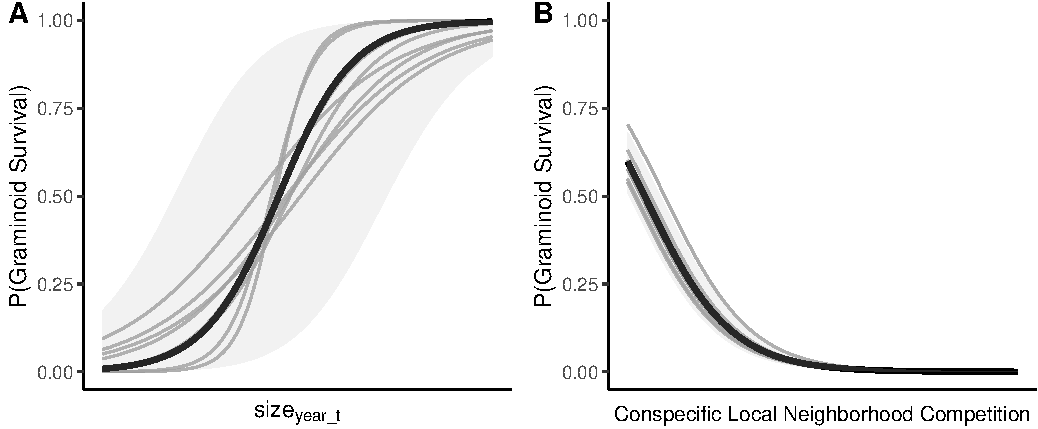
\includegraphics[width=.8\textwidth]{figures/survEffectPlots-1.pdf}
    \caption{The effect of size in year \textit{t} (\textbf{A}) and local neighborhood density (\textbf{B}) on graminoid survival in models using LDMC as the trait predictor. Dark lines indicate the overall effect of each covariate on survival. The 95\% confidence interval for the overall effect of each covariate is shown in light grey. Dark grey lines indicate the effects of each covariate according to species. For all measured graminoid species, larger individuals are more likely to survive to the next year than smaller individuals of the same species (\textbf{A}). Across all graminoid species, higher crowding of an individual's local neighborhood (10 cm radius) with individuals of the same species corresponds to lower survival probability (\textbf{B}). }
    \label{fig:Effects_Survival}
\end{figure}

\section{Discussion}
The effect of trait values on \textbf{survival} varies according to drought intensity for species in this shortgrass steppe ecosystem. This supports our hypothesis that water-related traits mediate the effect of drought on plant demographic rates, and the pattern of this mediation differs depending on drought severity. Although the strength of the interactions between trait values and drought varies according to functional group and the trait in question (Table \ref{ModResults}; Table \ref{ForbSurv_ModResults}), the fact that the interaction is significant in most cases indicates that this question merits further study, particularly for traits that are functionally related to the most limiting resources in a given habitat. 

The interaction we identified between water-related traits and SPEI does, however, differ somewhat from our predictions. We predicted consistently high survival probability in wet years regardless of a species' position along a spectrum for any given trait. In dry years, we expected high survival for high LDMC and low TLP species and low survival for high TLP and low LDMC species (Fig. \ref{fig:PredsObs} a-b). The modeled survival probabilities in dry years are consistent with our expectations across the spectrum of values for TLP and LDMC. However in wet years, survival probability is not consistently high. Instead, survival declines for low TLP and high LDMC species (Fig. \ref{fig:PredsObs} c-f). This pattern could indicates a trade-off between competitive ability and drought tolerance. Species with low TLP and high LDMC are more likely to survive in dry years, but have lower survival in wet years because they are more likely to be out-competed by their neighbors with high TLP and low LDMC that are more abundant. A substantial body of literature supports the existence of a trade-off between stress-tolerance and competitive ability \citep{Grime1979, Grime1997, Craine2007, Volaire2018}, but further analysis of this dataset might provide more direct evidence of this phenomenon in this particular shortgrass steppe ecosystem. 

The effect of drought intensity on \textbf{growth} is not significantly mediated by functional traits, regardless of the trait in question (Table \ref{growth_ModResults}). This result might suggest that the environmental filter \citep{HilleRisLambers2012} of drought is strong in this habitat, such that in dry years, species that lie on the low end of a spectrum of drought tolerance are unlikely to survive. Those species that do survive drought uniformly grow more in wet years than in dry years.   

We expected models using TLP to be better predictors of survival than models using LDMC or other, less explicitly water-related traits, but that is not the case in all situations. Both AIC values, as well as comparison of AIC for models without trait suggest that LDMC is actually a better predictor of survival than TLP. RDMC is possibly more predictive than TLP as well, although AIC values of models using TLP and RDMC cannot be compared because of different sample size. This result is encouraging from a methodological standpoint, since LDMC is substantially more efficient to measure than TLP. 

Collectively, these results provide evidence that plant functional traits related to water use can provide insight into the specific nature of the effect of drought on the vital rate process of survival. The lack of an interactive effect of drought and traits on growth is unexpected, but emphasizes the importance of testing this relationship in other habitats with varying patterns of annual average water availability. and constitutes an important test of the power of functional traits to predict demographic rates across a gradient of abiotic conditions.



\bibliography{references}

\section{Supplementary Information}

\begin{table}[h] \centering 
  \caption{Pearson correlation between traits for all species included in our analysis} 
  \label{allSppCorr}
\begin{tabular} {cccccccc} 
\\[-1.8ex]\hline 
\hline \\[-1.8ex] 
 & TLP & RootDiam & RTD & RDMC & SRL & LDMC & SLA \\ 
\hline \\[-1.8ex] 
\rowcolor[gray]{.95}TLP & $1$ & $0.281$ & $-$ $0.547$ & $-$ $0.653$ & $0.465$ & $-$ $0.760$ & $-$ $0.111$ \\ 
RootDiam &  & $1$ & $-$ $0.604$ & $-$ $0.553$ & $-$ $0.457$ & $-$ $0.477$ & $0.060$ \\ 
\rowcolor[gray]{.95}RTD& &  & $1$ & $0.881$ & $-$ $0.326$ & $0.836$ & $-$ $0.270$ \\ 
RDMC& & &  & $1$ & $-$ $0.404$ & $0.936$ & $-$ $0.047$ \\ 
\rowcolor[gray]{.95}SRL &  & &  & & $1$ & $-$ $0.476$ & $0.162$ \\ 
LDMC & &  & &  &  & $1$ & $-$ $0.145$ \\ 
\rowcolor[gray]{.95}SLA &  & & & & & & $1$ \\ 
\hline \\[-1.8ex] 
\end{tabular} 
\end{table}

\begin{figure}
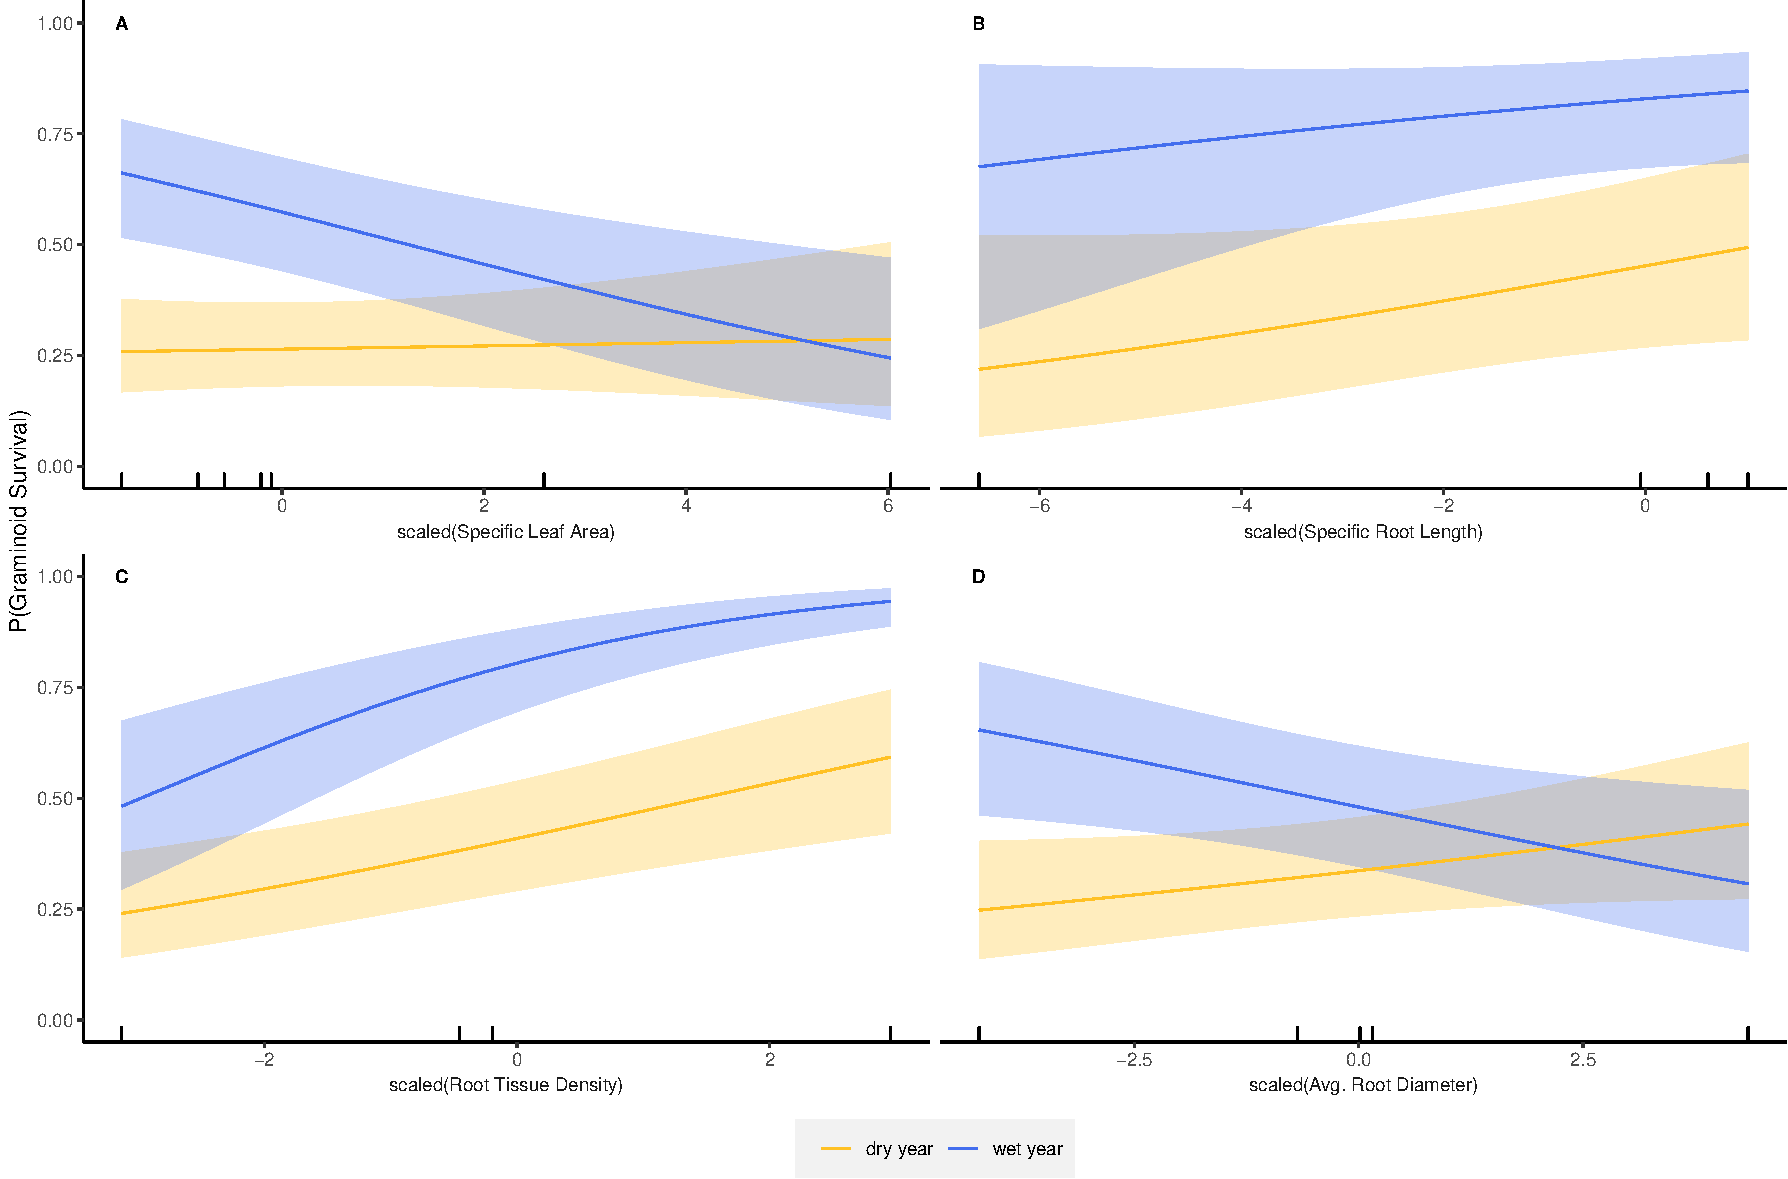
\includegraphics[width=.8\textwidth]{figures/supGramSurvPlots-1.pdf}
\caption{\small{
Illustration of the interaction between trait and SPEI for all graminoid survival models.
}}
\label{fig:GramSurv_all}
\end{figure}

\begin{figure}
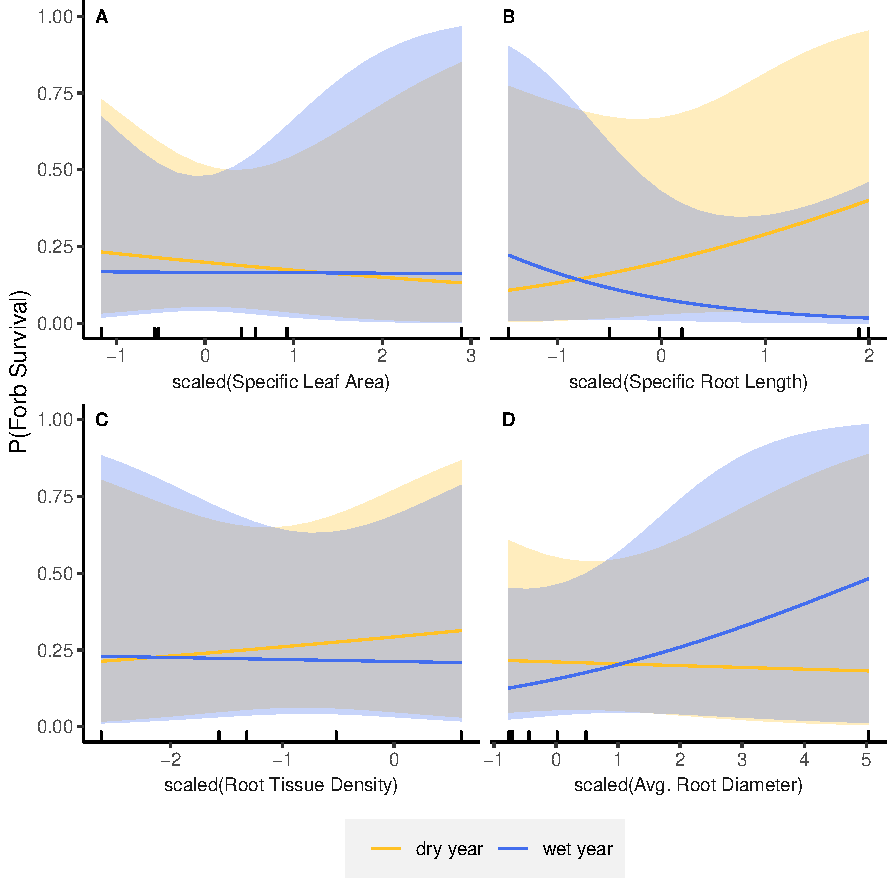
\includegraphics[width=.8\textwidth]{figures/supForbSurvPlots-1.pdf}
\caption{\small{
Illustration of the interaction between trait and SPEI for all forb survival models.
}}
\label{fig:ForbSurv_all}
\end{figure}

\begin{figure}
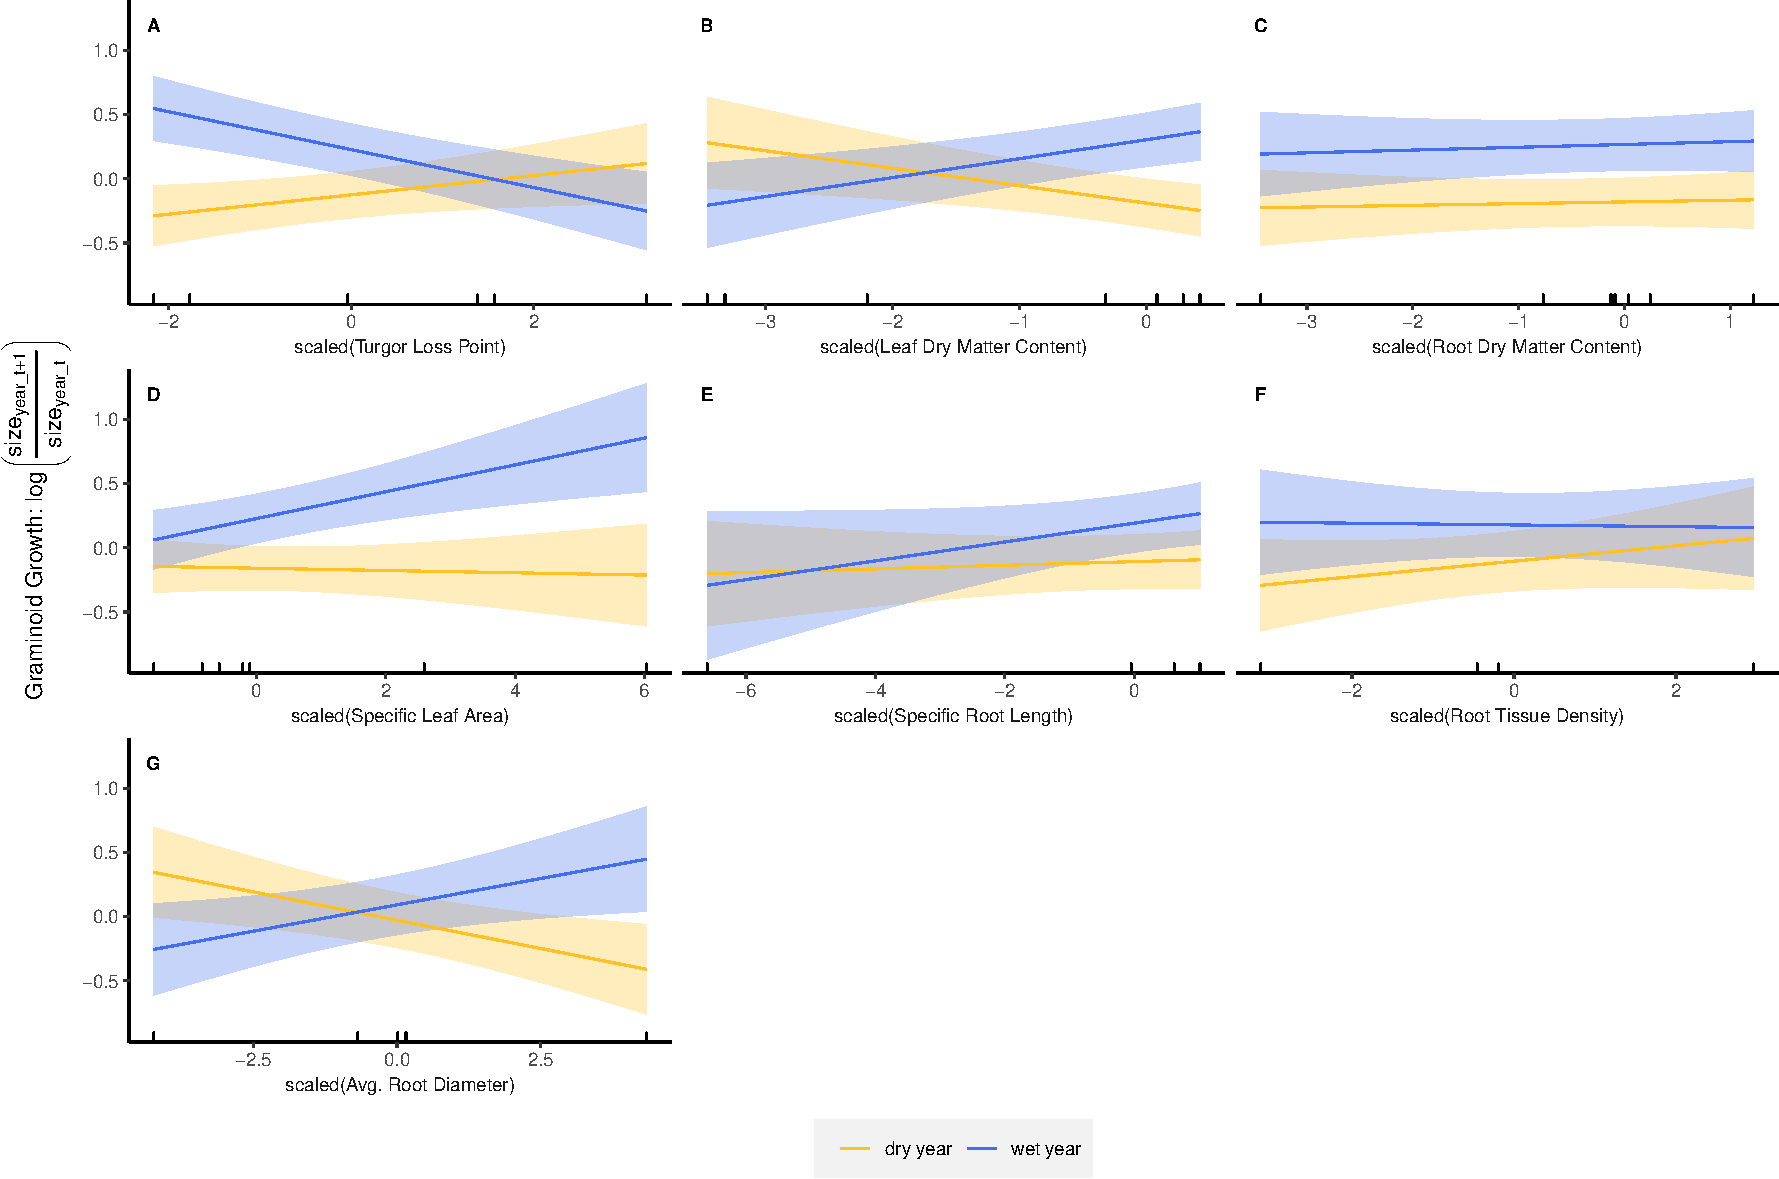
\includegraphics[width=1\textwidth]{figures/supGramGrowthPlots-1.pdf}
\caption{\small{
Illustration of the interaction between trait and SPEI for all graminoid models.
}}
\label{fig:Growth_all}
\end{figure}

\begin{figure}
    \centering
    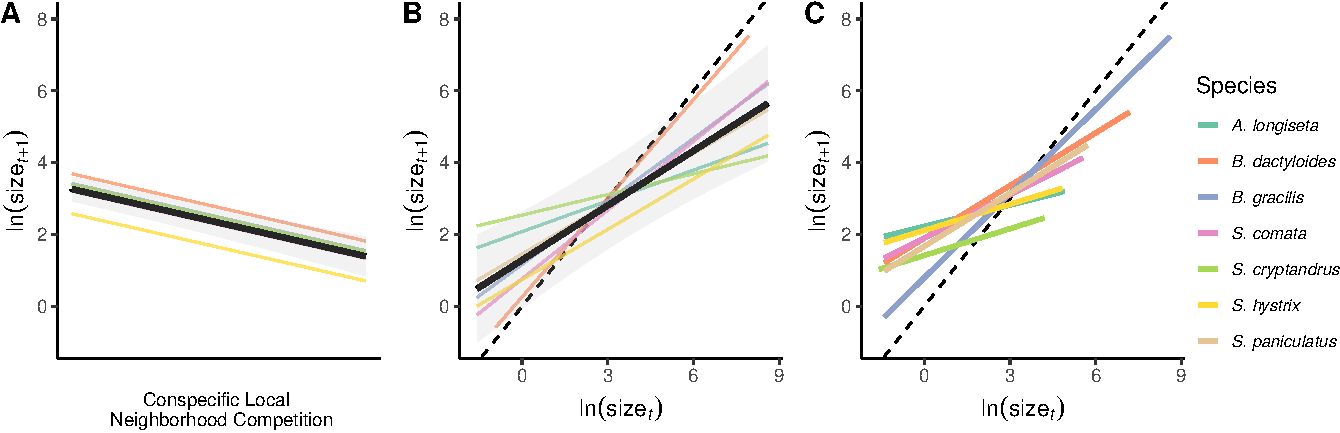
\includegraphics[width=.5\textwidth]{figures/growthEffectPlots-1.pdf}
    \caption{The effect of local neighborhood density on graminoid size in year \textit{t+1} in models using TLP as the trait predictor. Dark lines indicate the overall effect of each covariate on survival. The 95\% confidence interval for the overall effect of conspecific local neighborhood competition is shown in light grey. Dark grey lines indicate the effects of competition according to each species. Across all graminoid species, higher crowding of an individual's local neighborhood (10 cm radius) with individuals of the same species corresponds to lower growth in the next year.}
    \label{fig:Effects_Growth}
\end{figure}

\end{document}